\renewcommand{\imglabel}[1]{\put(2,85){\tiny\contour{black}{\textcolor{white}{\textbf{#1}}}}}
\begin{figure}[h!]
	\centering
	\setlength{\resLen}{0.115\columnwidth}
	\setlength{\raiseLen}{10pt}
	\addtolength{\tabcolsep}{-4.5pt}
	\footnotesize
	\begin{tabular}{ccccccccc}
		\raisebox{\raiseLen}{\rotatebox{90}{Photo}}
		&
		\begin{overpic}[width=\resLen]{bayesian/fig7/1_bump_3/target.jpg}
			\imglabel{Bump-3}
		\end{overpic}
		&
		\begin{overpic}[width=\resLen]{bayesian/fig7/2_leather_3/target.jpg}
			\imglabel{Leather-3}
		\end{overpic}
		&
		\begin{overpic}[width=\resLen]{bayesian/fig7/2_leather_6/target.jpg}
			\imglabel{Leather-6}
		\end{overpic}
		&
		\begin{overpic}[width=\resLen]{bayesian/fig7/3_plaster_3/target.jpg}
			\imglabel{Plaster-3}
		\end{overpic}
		&
		\begin{overpic}[width=\resLen]{bayesian/fig7/4_flake_4/target.jpg}
			\imglabel{Metallicflake-4}
		\end{overpic}
		&
		\begin{overpic}[width=\resLen]{bayesian/fig7/5_metal_3/target.jpg}
			\imglabel{Brushmetal-3}
		\end{overpic}
		&
		\begin{overpic}[width=\resLen]{bayesian/fig7/6_wood_3/target.jpg}
			\imglabel{Wood-3}
		\end{overpic}
		&
		\begin{overpic}[width=\resLen]{bayesian/fig7/6_wood_4/target.jpg}
			\imglabel{Wood-4}
		\end{overpic}
		\\
		\raisebox{\raiseLen}{\rotatebox{90}{Ours}} &
		\includegraphics[width=\resLen]{bayesian/fig7/1_bump_3/good1.jpg} &
		\includegraphics[width=\resLen]{bayesian/fig7/2_leather_3/good1.jpg} &
		\includegraphics[width=\resLen]{bayesian/fig7/2_leather_6/good1.jpg} &
		\includegraphics[width=\resLen]{bayesian/fig7/3_plaster_3/good1.jpg} &
		\includegraphics[width=\resLen]{bayesian/fig7/4_flake_4/good1.jpg} &
		\includegraphics[width=\resLen]{bayesian/fig7/5_metal_3/good1.jpg} &
		\includegraphics[width=\resLen]{bayesian/fig7/6_wood_3/good1.jpg} &
		\includegraphics[width=\resLen]{bayesian/fig7/6_wood_4/good1.jpg}
		\\
		\raisebox{\raiseLen}{\rotatebox{90}{[Hu '19]}} &
		
\includegraphics[width=\resLen]{bayesian/fig10/1_bump_3/00.jpg} &
		
\includegraphics[width=\resLen]{bayesian/fig10/2_leather_3/00.jpg} &
		
\includegraphics[width=\resLen]{bayesian/fig10/2_leather_6/00.jpg} &
		
\includegraphics[width=\resLen]{bayesian/fig10/3_plaster_3/00.jpg} &
		
\includegraphics[width=\resLen]{bayesian/fig10/4_flake_4/00.jpg} &
		
\includegraphics[width=\resLen]{bayesian/fig10/5_metal_3/00.jpg} &
		
\includegraphics[width=\resLen]{bayesian/fig10/6_wood_3/00.jpg} &
		
\includegraphics[width=\resLen]{bayesian/fig10/6_wood_4/00.jpg}
		\\[-10pt]
	\end{tabular}
	\caption[Comparison to Hu et al]{\label{fig:bayesian:hu}
		\textbf{Comparison} to the forward neural prediction method of Hu et al. \cite{hu2019novel}, where we apply their network structure with our BRDFs and lighting conditions. The photo (top) is better matched by our MCMC sampling results (middle) than their prediction (bottom), which moreover tends to become worse for more complex BRDF models and with more parameters. On the other hand, \cite{hu2019novel} can be used as an efficient initialization of our sampling, as shown in Figure \ref{fig:bayesian:hu2}.
	}
\end{figure}
